\documentclass[12pt]{report}

% Import packages from local file
\usepackage{packages}

% Define the homework number as a variable
\newcommand{\HomeworkNumber}{1}

\begin{document}


% Add the cover


% Set up custom date format
\newdateformat{monthyeardate}{\monthname[\THEMONTH] \THEYEAR}

% Header and Footer configuration
\pagestyle{fancy}
\fancyhf{}
\fancyhead[L]{\leftmark}
\fancyhead[R]{\thepage}
\fancyfoot[C]{Probabilistic Modeling and Reasoning Homework \HomeworkNumber}

% Chapter and Section formatting
\titleformat{\chapter}[display]
  {\normalfont\bfseries}{}{0pt}{\Huge}
\titlespacing*{\chapter}{0pt}{-20pt}{20pt}

% Adjust header height and top margin
\setlength{\headheight}{14.49998pt}
\addtolength{\topmargin}{-2.49998pt}

% % Custom abstract environment
% \newenvironment{customabstract}
%   {\vspace*{1cm}
%    \begin{center}
%    \bfseries \huge Abstract
%    \end{center}
%    \vspace{0.5cm}
%    \normalfont \large}
%   {\vspace{1cm}}



\makeatletter
% Taken from http://ctan.org/pkg/centernot
\newcommand*{\centernot}{%
  \mathpalette\@centernot
}
\def\@centernot#1#2{%
  \mathrel{%
    \rlap{%
      \settowidth\dimen@{$\m@th#1{#2}$}%
      \kern.5\dimen@
      \settowidth\dimen@{$\m@th#1=$}%
      \kern-.5\dimen@
      $\m@th#1\not$%
    }%
    {#2}%
  }%
}
\makeatother


\begin{titlepage}
    \centering

    % University logo
    \vfill
    \includegraphics[width=0.3\textwidth]{UOMLOGOEN.eps}
    \vfill

    % Main title
    {\Huge \textbf{Probabilistic Modeling and Reasoning}} \\
    {\LARGE Homework — \HomeworkNumber}

    \vfill  % Vertical fill for dynamic centering
    % Authors' names
    {\Large \textbf{Nikolaos Liouliakis (AID25001)}} \\
    {\Large \textbf{Vasileios-Efraim Tsavalia (AID25006)}}

    % \vfill

    % % Course submission information
    % {\Large A report submitted for the course} \\
    % {\Large \textbf{Probabilistic Modeling and Reasoning}}

    \vfill

    % Program and University information
    {\Large MSc in Artificial Intelligence and Data Analytics} \\
    {\Large University of Macedonia}

    \vfill

    % Supervisor information
    {\Large \textbf{Supervisor: Professor Dimitris Christou-Varsakelis}}

    \vfill

    % Date with custom format
    {\Large \monthyeardate\today} % Automatically displays in "October 2024" format
    
\end{titlepage}


\newpage


\section*{Problem 1}


\begin{figure}[H]
    \centering
    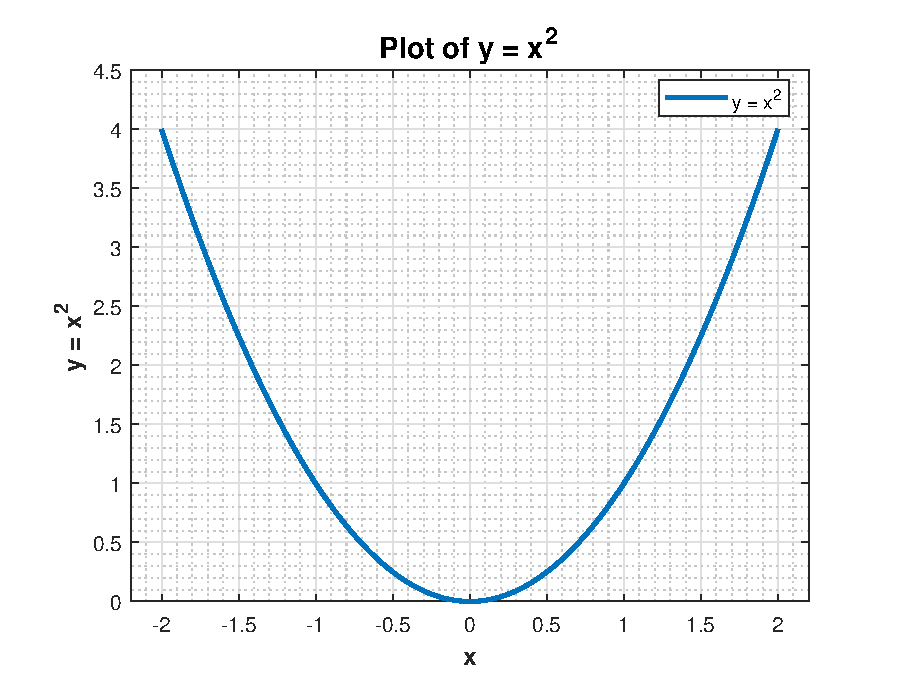
\includegraphics[width=0.75\linewidth]{y=x^2.eps}
    \caption{Plot of $y = x^2$.}
\end{figure}

% 2 Oct 2024 - 8 Oct 2024
% Dow Jones Industrial Average (^DJI)
% Nikkei 225 (^N225)
% DAX PERFORMANCE-INDEX (^GDAXI)
\begin{table}[H]
\centering
\label{tab:closing_prices_updated}
\begin{tabularx}{\textwidth}{Xrrrrr}
    \toprule
    \textbf{Index}     & \textbf{Day 1} & \textbf{Day 2} & \textbf{Day 3} & \textbf{Day 4} & \textbf{Day 5} \\
    \midrule
    DOW-JONES  & 42,080.37 & 41,954.24 & 42,352.75 & 42,011.59 & 42,196.52 \\
    NIKKEI     & 38,937.54 & 39,332.74 & 38,635.62 & 38,552.06 & 37,808.76 \\
    DAX        & 19,066.47 & 19,104.10 & 19,120.93 & 19,015.41 & 19,164.75 \\
    \bottomrule
\end{tabularx}
\caption{Closing prices of major stock indices over five days}
\end{table}



% Equations 

\begin{equation}
0 \leq P(A) \leq 1
\end{equation}

\begin{equation}
P(A^c) + P(A) = 1
\end{equation}

\begin{equation}
P(A \cup B) = P(A) + P(B) - P(A \cap B)
\end{equation}

\begin{equation}
P(A \cap B) = 0
\end{equation}

\begin{equation}
P(A \mid B) = \frac{P(A \cap B)}{P(B)}
\end{equation}

\begin{equation}
P(A \mid B) = \frac{P(B \mid A) \cdot P(A)}{P(B)}
\end{equation}

\begin{equation}
P(A \cap B) = P(A) \cdot P(B)
\end{equation}

\begin{equation}
F_X(x) = P(X \leq x)
\end{equation}

\begin{equation}
\sum_{i=1}^{n} P(X = x_i) = 1
\end{equation}

\begin{equation}
f_X(x) = \frac{dF_X(x)}{dx}
\end{equation}

\begin{equation}
F_X(x) = \int_{-\infty}^{x} f_X(y) \, dy
\end{equation}

\begin{equation}
F_X(x) = \sum_{i=1}^{n} P(X = k)
\end{equation}

\begin{equation}
P(a \leq X \leq b) = \int_{a}^{b} f_X(x) \, dx
\end{equation}

\begin{equation}
\int_{-\infty}^{\infty} f_X(x) \, dx = 1
\end{equation}

\begin{equation}
\text{Cov}(X, Y) = \mathbb{E}[(X - \mu_X)(Y - \mu_Y)] = \mathbb{E}[XY] - \mu_X \mu_Y
\end{equation}

\begin{equation}
\rho_{XY} = \frac{\text{Cov}(X,Y)}{\sigma_X \sigma_Y}
\end{equation}


\textbf{This is a sentence in boldface.} \\
\textit{This is a sentence in italics.}


\section*{Problem 2}

\subsection*{Part 1}
% Part 1 
Prove that

\begin{equation}
\Pr(x, y \mid z) = \Pr(x \mid z) \Pr(y \mid x, z)
\end{equation}


\begin{proof}

Left-hand side:

\begin{equation*}
\Pr(x, y \mid z) = \frac{\Pr(x, y, z)}{\Pr(z)} \nonumber \\[10pt]    
\end{equation*}

Right-hand side:

\begin{equation*}
\Pr(x \mid z) \Pr(y \mid x, z) = \frac{\Pr(x, z)}{\Pr(z)} \cdot \frac{\Pr(x, y, z)}{\Pr(x, z)} \nonumber \\[10pt]
= \frac{\Pr(x, y, z)}{\Pr(z)} \nonumber \\[10pt]
\end{equation*}

Since both sides are equal:

\begin{equation*}
\Pr(x, y \mid z) = \Pr(x \mid z) \Pr(y \mid x, z)
\end{equation*}

\end{proof}

\subsection*{Part 2}
% Part 2 
Prove that
\begin{equation}
\Pr(x \mid  y, z) = \frac{\Pr(y \mid x, z) \Pr(x \mid z)}{\Pr(y \mid z)}
\end{equation}

\begin{proof}

Left-hand side:

\begin{equation*}
\Pr(x \mid  y, z) = \frac{\Pr(x, y, z)}{\Pr(y,z)}
\end{equation*}

Right-hand side:

\begin{equation*}
\frac{\Pr(y \mid x, z) \Pr(x \mid z)}{\Pr(y \mid z)} = \frac{\frac{\Pr(x, y, z)}{\Pr(x,z)} \frac{\Pr(x, z)}{\Pr(z)}}{\frac{\Pr(y, z)}{\Pr(z)}} 
= \frac{\Pr(x, y, z)}{\Pr(y,z)}
\end{equation*}

Since both sides are equal:

\begin{equation*}
\Pr(x, y \mid z) = \Pr(x \mid z) \Pr(y \mid x, z)
\end{equation*}

\end{proof}


\section*{Problem 3}

We are given:

\begin{itemize}
    \item Box 1 contains 3 red and 5 white balls.
    \item Box 2 contains 2 red and 5 white balls.
    \item A box is chosen at random, so \( \Pr(\text{box 1}) = \Pr(\text{box 2}) = 0.5 \).
    \item A red ball is chosen, and we want to find the Probability that it came from box 1.
\end{itemize}

We apply Bayes' theorem:

\[
\Pr(\text{box 1} \mid \text{red}) = \frac{\Pr(\text{red} \mid \text{box 1}) \cdot \Pr(\text{box 1})}{\Pr(\text{red})}
\]

Where:
\[
\Pr(\text{red} \mid \text{box 1}) = \frac{3}{3+5} = \frac{3}{8}, \quad \Pr(\text{red} \mid \text{box 2}) = \frac{2}{2+5} = \frac{2}{7}
\]
and
\[
\Pr(\text{red}) = \Pr(\text{red} \mid \text{box 1}) \cdot \Pr(\text{box 1}) + \Pr(\text{red} \mid \text{box 2}) \cdot \Pr(\text{box 2})
\]
Substitute the known values:
\[
\Pr(\text{red}) = \left(\frac{3}{8} \cdot 0.5\right) + \left(\frac{2}{7} \cdot 0.5\right) = \frac{3}{16} + \frac{2}{14} = \frac{37}{112}
\]

Now, applying Bayes' theorem:

\[
\Pr(\text{box 1} \mid \text{red}) = \frac{\frac{3}{8} \cdot 0.5}{\frac{37}{112}} = 0.567
\]

Thus, the posterior probability that the red ball came from box 1 is approximately \( 0.568 \) or 56.8\%.



\section*{Problem 4}

We are provided with the following information:

\begin{itemize}
    \item There is exactly one terrorist on the plane, and there are 100 passengers.
    \item The scanner has a true positive rate of 95\% (i.e., it correctly identifies terrorists 95\% of the time).
    \item The scanner has a true negative rate of 95\% (i.e., it correctly identifies upstanding citizens 95\% of the time).
    \item We scan the passengers one by one until we find the first positive result.
\end{itemize}


% \subsubsection*{Outline of the solution}

The idea is to consider all the possible cases where the terrorist is seated in the k-th seat (for k=1,2,…,100), and sum over these cases. In particular, for the terrorist to be the person identified as the terrorist when sitting in seat k, the following must happen:

\begin{enumerate}
    \item The first $k-1$ people must test negative (since they are all upstanding citizens).
    \item The person in the k-th seat (the terrorist) must test positive.
\end{enumerate}

Let $P(K=k)$ be the event that the terrorist is in the k-th seat.

\begin{equation*}
P(K=k) = \frac{1}{100}, \quad k = 1, 2, \dots, 100
% \Pr(\text{Terrorist in seat k}) = \frac{1}{100}
\end{equation*}

Now, let $P(FP = 1 , K=k)$ be the joint probability that the terrorist is in the $k$-th seat, is the first to test positive and is correctly identified. 

\begin{equation*}
P(FP = 1 , K=k) = P(FP = 1 \mid K=k) P(K=k)
\end{equation*}


% \begin{equation*}
% \Pr(\text{First $k-1$ scans are negative} \mid \text{Terrorist in seat k}) = 0.95^{k-1}
% \end{equation*}

% \begin{equation*}
% \Pr(\text{The k-th scan is possitive} \mid \text{Terrorist in seat k}) = 0.95
% \end{equation*}


\begin{equation*}
P(FP = 1 \mid K=k) = 0.95^{k-1} \cdot 0.95 = 0.95^k
\end{equation*}

Using the law of total probability $P(FP=1)$ is expressed as:
\begin{equation*}
P(FP=1) = \sum_{k = 1}^{100} P(FP = 1 \mid K=k) \cdot P(K=k)
\end{equation*}


\begin{equation*}
P(FP=1) = \sum_{k = 1}^{100} 0.95^{k} \frac{1}{100}  
\end{equation*}

\begin{equation*}
P(FP=1) \simeq  0.1889
\end{equation*}

Therefore, the probability that the first person to test positive is, indeed, a terrorist is $18.89\%$

\section*{Problem 5}


\begin{figure}[H]
    \centering
    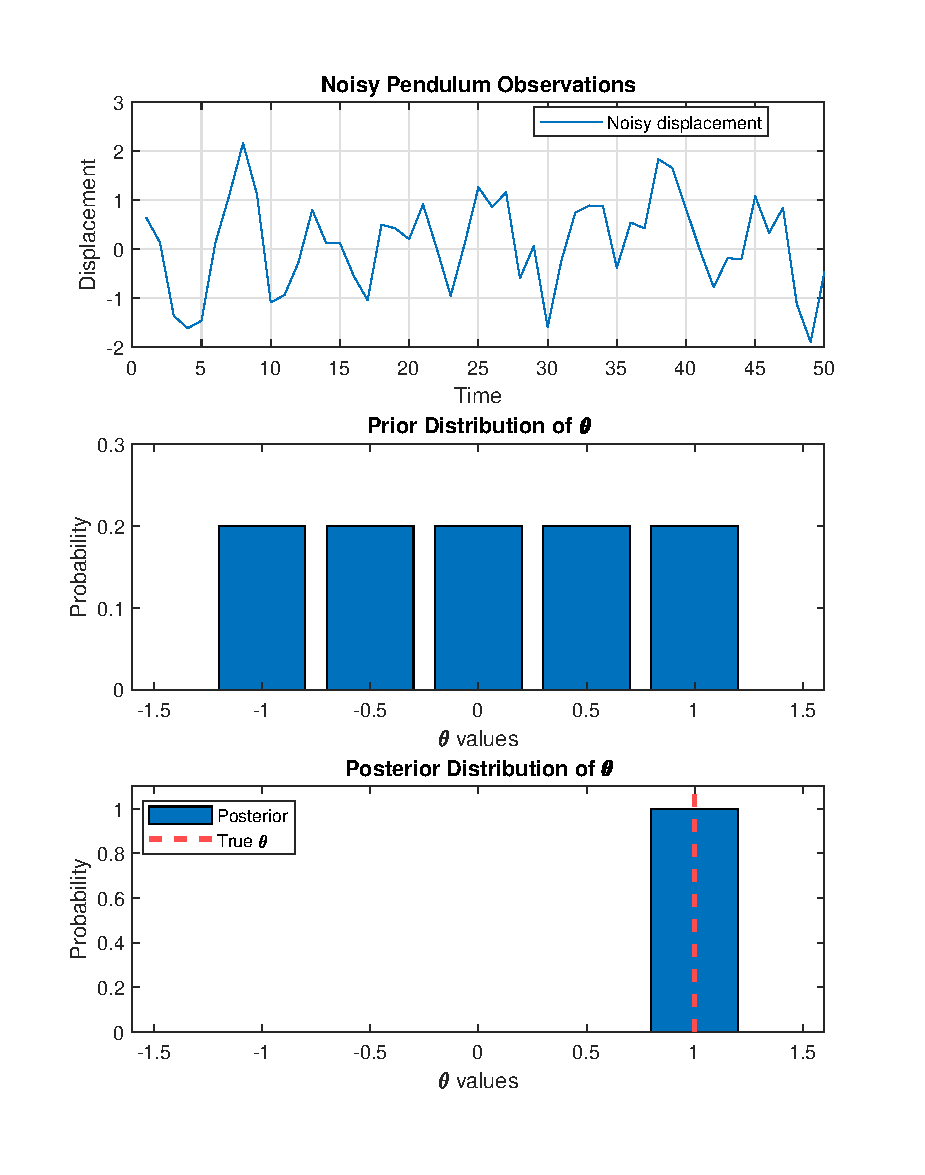
\includegraphics[width=0.75\linewidth]{pendulum.eps}
    \caption{Diagram produced by code}
\end{figure}



\section*{Problem 6}

% \textbf{Given Data}

Prior distribution of \(\theta\):
  \[
  \theta \sim \mathcal{N}(\mu_{\text{prior}}, \sigma_{\text{prior}}^2)
  \]
  
Observations \(y_i\) are generated as:
  \[
  y_i = \theta + \sigma_y \nu_i, \quad \nu_i \sim \mathcal{N}(0,1)
  \]

\[
\mathbb{E}[Y] = \mathbb{E}[\theta + \sigma_y \nu_i] = \theta + \sigma_y \mathbb{E}[\nu_i] = \theta
\]

\[
\text{Var}(Y) = \text{Var}(\theta + \sigma_y \nu_i) = \text{Var}(\sigma_y \nu_i) = \sigma_y^2 \text{Var}(\nu_i) = \sigma_y^2
\]


Therefore 
\[
Y \sim \mathcal{N}(\theta, \sigma_y^2)
\]






% \textbf{Likelihood:}

Assuming that the measurements are independent, the likelihood for a sequence of observations \( y_1, y_2, \ldots, y_N \) is:
\[
p(y_1, \ldots, y_N | \theta) = \prod_{i=1}^{N} p(y_i | \theta)
\]

Each observation follows a normal distribution, so:
\[
p(y_i | \theta) = \frac{1}{\sqrt{2 \pi \sigma_y^2}} \exp \left( -\frac{(y_i - \theta)^2}{2 \sigma_y^2} \right)
\]

Thus, the likelihood for the sequence is:
\[
p(y_1, \ldots, y_N | \theta) = \left( \frac{1}{\sqrt{2 \pi \sigma_y^2}} \right)^N \exp\left( -\frac{1}{2 \sigma_y^2} \sum_{i=1}^{N} (y_i - \theta)^2 \right)
\]

% \textbf{Posterior:}

The posterior distribution is:
\[
p(\theta | y_1, \ldots, y_N) \propto p(y_1, \ldots, y_N | \theta) p(\theta)
\]

Substituting the likelihood and prior:
\[
p(\theta | y_1, \ldots, y_N) \propto \left( \frac{1}{\sqrt{2 \pi \sigma_y^2}} \right)^N \exp\left( -\frac{1}{2 \sigma_y^2} \sum_{i=1}^{N} (y_i - \theta)^2 \right)
\frac{1}{\sqrt{2 \pi \sigma_{\text{prior}}^2}} \exp \left( -\frac{(\mu_{\text{prior}} - \theta)^2}{2 \sigma_{\text{prior}}^2} \right)
\]

% After the sum 
\[
p(\theta | y_1, \ldots, y_N) \propto  \exp\left( -\frac{1}{2 \sigma_y^2} \sum_{i=1}^{N} (y_i - \theta)^2  -\frac{(\mu_{\text{prior}} - \theta)^2}{2 \sigma_{\text{prior}}^2} \right)
\]


\begin{equation}
p(\theta | y_1, \ldots, y_N) \propto  \exp\left( -\frac{1}{2}    
\left[  
\left( \frac{1}{\sigma_{\text{prior}}^2} + \frac{N}{\sigma_y^2} \right) \theta^2    
- 2 \left( \frac{\mu_{\text{prior}}}{\sigma_{\text{prior}}^2} + \frac{\sum_{i=1}^N y_i}{\sigma_y^2} \right) \theta 
+ \frac{\mu_{\text{prior}}^2}{\sigma_{\text{prior}}^2}+ \frac{\sum_{i=1}^N y_i^2}{\sigma_y^2}
\right] 
\right)    
\end{equation}

Since we know 

\[
p(\theta | y_1, \ldots, y_N) \sim \mathcal{N}(\mu_{\text{post}}, \sigma_{\text{post}}^2)
\]

\begin{align}    
p(\theta | y_1, \ldots, y_N) &= \frac{1}{\sqrt{2 \pi \sigma_{\text{post}}^2}} \exp \left( -\frac{(\mu_{\text{post}} - \theta)^2}{2 \sigma_{\text{post}}^2} \right)
\\
&= \frac{1}{\sqrt{2 \pi \sigma_{\text{post}}^2}} \exp \left( - \frac{1}{2}
\left[
\frac{1}{\sigma_{\text{post}}^2} \theta^2
- 2 \frac{\mu_{\text{post}}}{\sigma_{\text{post}}^2} \theta
+ \frac{\mu_{\text{post}}^2}{\sigma_{\text{post}}^2}
\right] 
\right)
\end{align}


% Result
By equating the polynomial coefficients of the terms involving $\theta$ in the exponent, we can calculate the posterior mean and variance for $\theta$ after N observations.


\begin{equation}
\mu_{\text{post}} = \sigma_{\text{post}}^2 \left( \frac{\mu_{\text{prior}}}{\sigma_{\text{prior}}^2} + \frac{\sum_{i=1}^N y_i}{\sigma_y^2} \right)
\end{equation}


\begin{equation}    
\sigma_{\text{post}}^2 = \left( \frac{1}{\sigma_{\text{prior}}^2} + \frac{N}{\sigma_y^2} \right)^{-1}
\end{equation}


With \(\mu_{\text{prior}} = 1\) , \(\sigma_{\text{prior}}^2 = 2\) , \(\sigma_y = 0.5\) and only one observation \(y_1 = -1\), we have:


\begin{equation*}    
\sigma_{\text{post}}^2 = \left( \frac{1}{2^2} + \frac{1}{0.5^2} \right)^{-1} = \frac{4}{17} \approx 0.2353
\end{equation*}


\begin{equation*}
\mu_{\text{post}} = \frac{4}{17} \left( \frac{1}{2^2} + \frac{-1}{0.5^2} \right) = -\frac{15}{17} \approx -0.882
\end{equation*}

\end{document}
